% -------------------- Result and Analysis ----------------------------------

\pagebreak

\section{Results and Analysis}
%Prepare the test plans in tabular format, where each Test Case should be represented with distinct id, prefixed with “$\langle$module$\rangle$ “, where module represents the short code of the respective design module. Test Case numbers should be matching as stated in Requirement Matrix.
%\vspace{.1in}

%\noindent

%Appropriate definition of ‘Performance Metrics’, e.g. Classification Accuracy, Mean Squared Error etc. should be included, as applicable. 
%\vspace{.1in}

%\noindent
%Depending on your specific project, test results can be represented as a table of data with a corresponding pie chart / bar chart as needed. Analysis of test results should be discussed in terms of clear bullet points.

\noindent
The metrics used for evaluating the performance of the classification models include Precision, Recall, F1-Score, and Support, along with the Confusion Matrix. These metrics are crucial for assessing how well the models are able to differentiate between various classes, providing insight into their accuracy, ability to capture relevant instances, and the overall balance between precision and recall. By analyzing these metrics, a comprehensive understanding of the model's performance can be obtained, enabling informed decisions for further optimization and tuning.

\subsection{Classification Metrics and Confusion Matrix}

\begin{itemize}
    \item \textbf{Precision:} Precision is the ratio of correctly predicted positive observations to the total predicted positives. It can be calculated as:
    \[
    \text{Precision} = \frac{TP}{TP + FP}
    \]
    where \( TP \) represents True Positives, and \( FP \) represents False Positives.

    \item \textbf{Recall:} Recall is the ratio of correctly predicted positive observations to all observations in the actual class:
    \[
    \text{Recall} = \frac{TP}{TP + FN}
    \]
    where \( TP \) is True Positives, and \( FN \) is False Negatives.

    \item \textbf{F1-Score:} F1-Score is the harmonic mean of Precision and Recall, calculated as:
    \[
    \text{F1-Score} = 2 \times \frac{\text{Precision} \times \text{Recall}}{\text{Precision} + \text{Recall}}
    \]

    \item \textbf{Support:} Support refers to the number of actual occurrences of each class in the dataset:
    \[
    \text{Support} = \text{Number of samples in the true class}
    \]

    \item \textbf{Confusion Matrix:} A confusion matrix is used to evaluate the performance of a classification model. It is structured as follows:
    \[
    \begin{bmatrix}
    TP & FP \\
    FN & TN
    \end{bmatrix}
    \]
    where:
    \begin{itemize}
        \item \( TP \) = True Positives
        \item \( FP \) = False Positives
        \item \( FN \) = False Negatives
        \item \( TN \) = True Negatives
    \end{itemize}
\end{itemize}

\subsection{Results of Logistic Regression}

\begin{center}
    \textbf{Logistic Regression Classification Report} \\[0.5em]
    \begin{tabular}{|l|c|c|c|c|}
        \hline
        \textbf{Class} & \textbf{Precision} & \textbf{Recall} & \textbf{F1-Score} & \textbf{Support} \\ \hline
        Anxiety        & 0.83               & 0.77            & 0.80              & 379              \\ \hline
        Bipolar        & 0.74               & 0.55            & 0.63              & 384              \\ \hline
        Depression     & 0.76               & 0.76            & 0.76              & 373              \\ \hline
        Normal         & 0.92               & 0.99            & 0.95              & 2183             \\ \hline
        PTSD           & 0.87               & 0.77            & 0.82              & 394              \\ \hline
        \textbf{Accuracy} & \multicolumn{4}{|c|}{87.66\%} \\ \hline
        \textbf{Macro Avg} & 0.82            & 0.77            & 0.79              & 3713             \\ \hline
        \textbf{Weighted Avg} & 0.87         & 0.88            & 0.87              & 3713             \\ \hline
    \end{tabular}
\end{center}

\vspace{0.25em}

\begin{center}
    \textbf{Confusion Matrix for Logistic Regression Model} \\[0.5em]
    \begin{tabular}{|c|c|c|c|c|c|}
        \hline
        & \textbf{Anxiety} & \textbf{Bipolar} & \textbf{Depression} & \textbf{Normal} & \textbf{PTSD} \\ \hline
        \textbf{Anxiety}    & 291 & 18  & 27  & 24  & 19  \\ \hline
        \textbf{Bipolar}    & 7   & 213 & 29  & 125 & 10  \\ \hline
        \textbf{Depression} & 26  & 31  & 283 & 18  & 15  \\ \hline
        \textbf{Normal}     & 3   & 10  & 4   & 2165 & 1   \\ \hline
        \textbf{PTSD}       & 24  & 16  & 29  & 22  & 303 \\ \hline
    \end{tabular}
\end{center}

\vspace{0.25em}

\begin{center}
    \textbf{ROC Curve Areas for Each Class} \\[0.5em]
    \begin{tabular}{|l|c|}
        \hline
        \textbf{Class}  & \textbf{ROC AUC} \\ \hline
        Anxiety         & 0.95            \\ \hline
        Bipolar         & 0.92            \\ \hline
        Depression      & 0.96            \\ \hline
        Normal          & 0.99            \\ \hline
        PTSD            & 0.95            \\ \hline
    \end{tabular}
\end{center}

\vspace{0.25em}

\noindent
The Logistic Regression model performed well with an overall accuracy of 87.66\%, indicating that the model correctly classified the majority of the instances. The classification report shows high precision, recall, and F1-scores for the 'Normal' class, which was expected due to its large number of instances. However, the 'Bipolar' and 'Anxiety' classes have lower recall and F1-scores, suggesting that the model struggles more with these classes. The confusion matrix highlights the misclassifications. For example, 'Anxiety' is often confused with 'Depression' and 'PTSD,' while the 'Normal' class is well-separated from the other classes. The large number of instances in the 'Normal' class could have contributed to the high accuracy but also to the imbalance in performance across other classes. The ROC curve AUC scores indicate that the model performs well in distinguishing between the classes. The 'Normal' class has the highest AUC (0.99), which is expected due to the large proportion of 'Normal' instances. Other classes, like 'Anxiety' and 'Depression,' also have high AUC scores (0.95 and 0.96, respectively), indicating that the model is capable of distinguishing them effectively.


\begin{figure}[h!]  
    \centering
    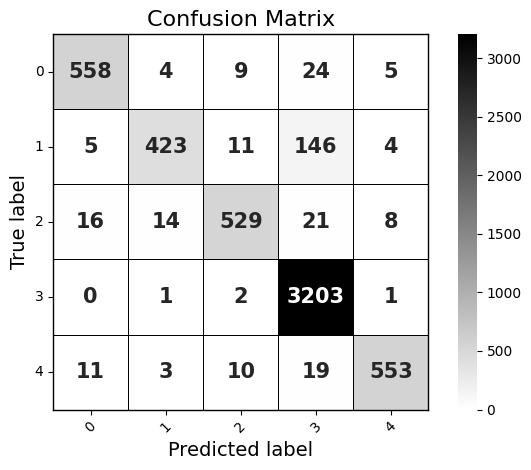
\includegraphics[width=0.8\textwidth]{Images/LR Confusion Matrix.png}  
    \caption{Confusion Matrix (Logistic Regression)}
    \label{LRCM}  % Label for referencing the figure
\end{figure}

\begin{figure}[h!]  
    \centering
    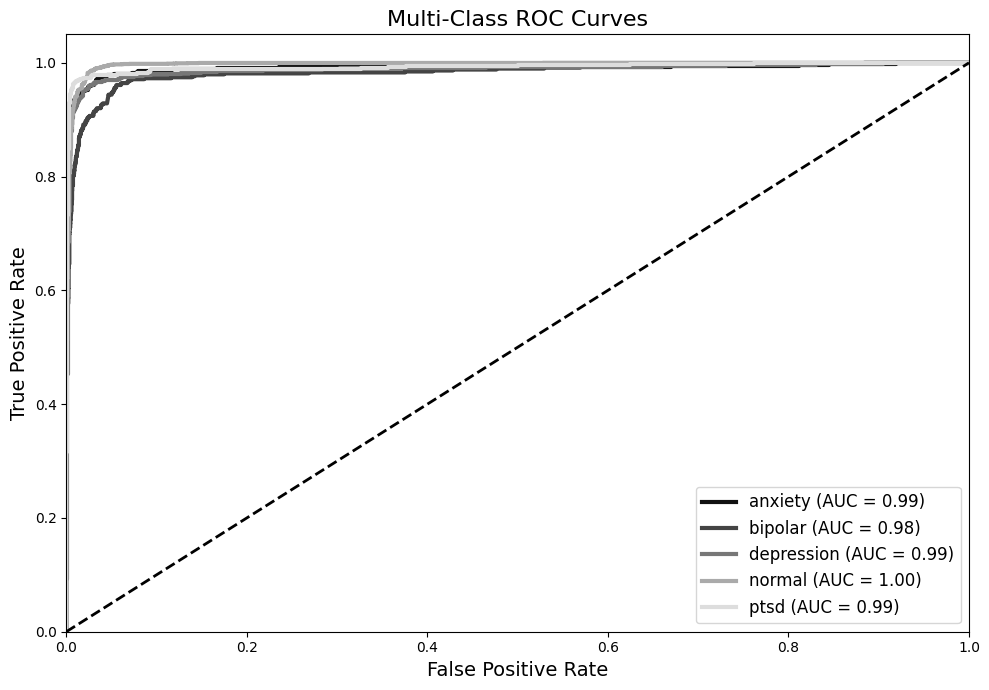
\includegraphics[width=0.85\textwidth]{Images/LR ROC.png}  
    \caption{ROC AUC (Logistic Regression)}
    \label{LRROC}  % Label for referencing the figure
\end{figure}


\subsection{Results of Naive Bayes}

\begin{center}
    \textbf{Naive Bayes Classification Report} \\[0.5em]
    \begin{tabular}{|l|c|c|c|c|}
        \hline
        \textbf{Class} & \textbf{Precision} & \textbf{Recall} & \textbf{F1-Score} & \textbf{Support} \\ \hline
        Anxiety        & 0.70               & 0.73            & 0.72              & 379              \\ \hline
        Bipolar        & 0.83               & 0.45            & 0.58              & 384              \\ \hline
        Depression     & 0.59               & 0.87            & 0.70              & 373              \\ \hline
        Normal         & 0.96               & 0.92            & 0.94              & 2183             \\ \hline
        PTSD           & 0.71               & 0.83            & 0.76              & 394              \\ \hline
        \textbf{Accuracy} & \multicolumn{4}{|c|}{83.63\%} \\ \hline
        \textbf{Macro Avg} & 0.76            & 0.76            & 0.74              & 3713             \\ \hline
        \textbf{Weighted Avg} & 0.85         & 0.84            & 0.84              & 3713             \\ \hline
    \end{tabular}
\end{center}

\vspace{0.25em}

\begin{center}
    \textbf{Confusion Matrix for Naive Bayes Model} \\[0.5em]
    \begin{tabular}{|c|c|c|c|c|c|}
        \hline
        & \textbf{Anxiety} & \textbf{Bipolar} & \textbf{Depression} & \textbf{Normal} & \textbf{PTSD} \\ \hline
        \textbf{Anxiety}    & 278 & 4    & 63  & 3    & 31    \\ \hline
        \textbf{Bipolar}    & 30  & 171  & 62  & 86   & 35    \\ \hline
        \textbf{Depression} & 26  & 6    & 323 & 0    & 18    \\ \hline
        \textbf{Normal}     & 38  & 21   & 68  & 2006 & 50    \\ \hline
        \textbf{PTSD}       & 24  & 5    & 34  & 4    & 327   \\ \hline
    \end{tabular}
\end{center}

\vspace{0.25em}
\pagebreak
\begin{center}
    \textbf{ROC Curve Areas for Each Class} \\[0.5em]
    \begin{tabular}{|l|c|}
        \hline
        \textbf{Class}  & \textbf{ROC AUC} \\ \hline
        Anxiety         & 0.92            \\ \hline
        Bipolar         & 0.89            \\ \hline
        Depression      & 0.94            \\ \hline
        Normal          & 0.99            \\ \hline
        PTSD            & 0.94            \\ \hline
    \end{tabular}
\end{center}

\vspace{0.25em}

\begin{figure}[h!]  
    \centering
    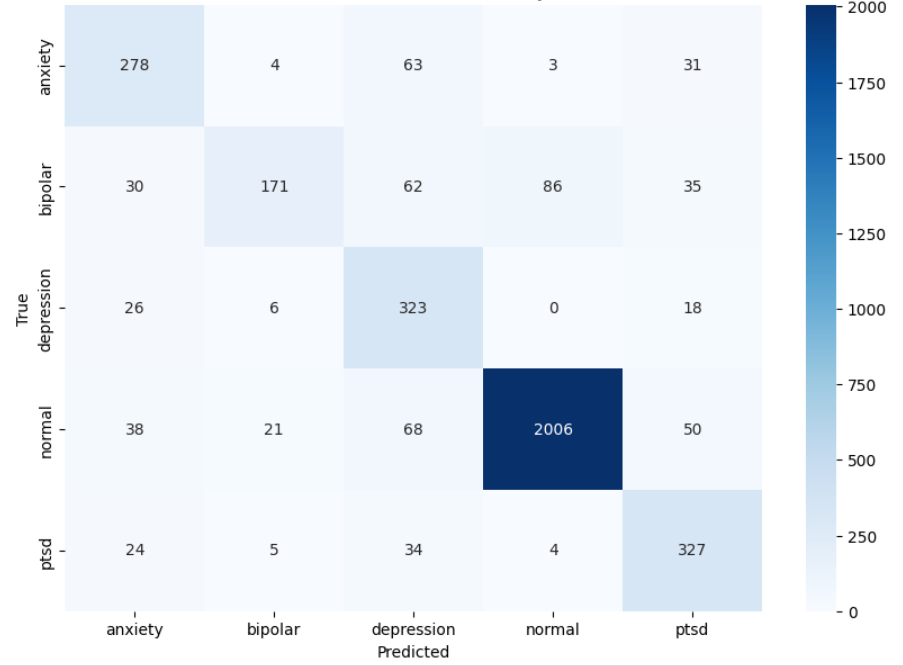
\includegraphics[width=0.8\textwidth]{Images/NB Confusion Matrix.png}  
    \caption{Confusion Matrix (Naive Bayes)}
    \label{NBCM}  % Label for referencing the figure
\end{figure}

\noindent
The Naive Bayes model achieved an overall accuracy of 83.63\%, indicating a reasonable performance. The classification report shows strong results for the Normal class, with a precision of 0.96 and a recall of 0.92, resulting in an F1-score of 0.94. However, the Bipolar class exhibits much lower recall (0.45) and F1-score (0.58), suggesting that the model struggles to accurately identify Bipolar instances. Misclassifications are more frequent for Bipolar, often being confused with Depression and PTSD. The Anxiety class, although having decent precision (0.70), shows a lower recall (0.73), indicating that it also faces challenges in classification. The Confusion Matrix highlights that the model has difficulty distinguishing Bipolar and Depression from each other, with a large number of misclassifications across these classes. On the other hand, the Normal class is well-separated and correctly classified, with 2006 true positives, which likely contributes to the high overall accuracy. PTSD also shows relatively good classification results, with misclassifications being less frequent. The ROC AUC Curve Areas show that the model performs well for most classes, with the Normal class having the highest AUC score (0.99), followed by Depression and PTSD with AUCs of 0.94. While the model performs well for distinguishing between classes like Normal and Depression, the lower AUC for Bipolar (0.89) indicates that there may still be room for improvement in distinguishing this class from others.



\begin{figure}[h!]  
    \centering
    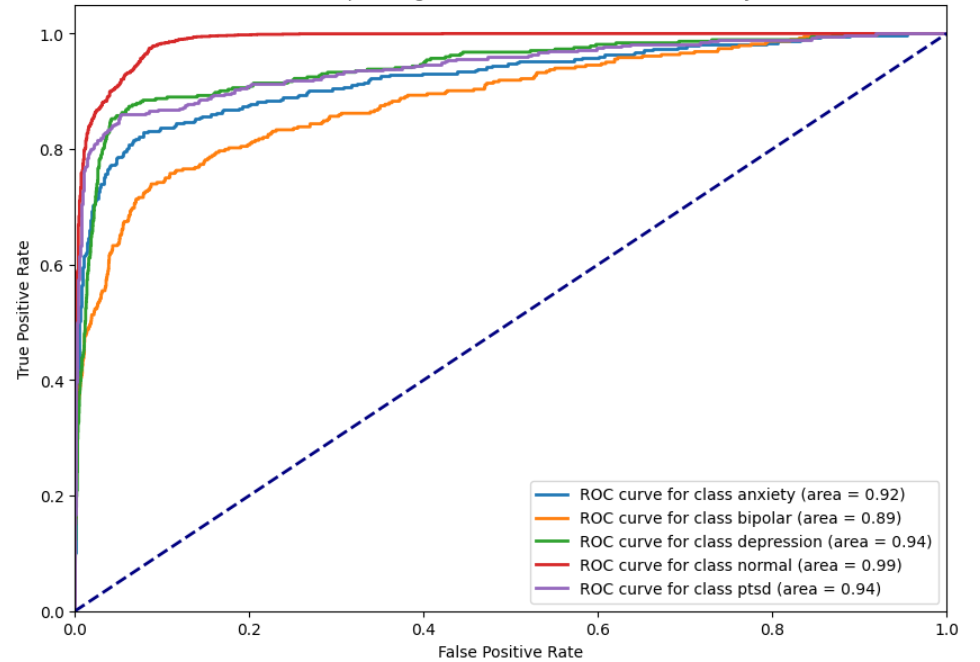
\includegraphics[width=0.75\textwidth]{Images/NB ROC.png}  
    \caption{ROC AUC (Naive Bayes)}
    \label{NBROC}  % Label for referencing the figure
\end{figure}


\subsection{Results of Support Vector Machine}

\begin{center}
    \textbf{SVM Classification Report} \\[0.5em]
    \begin{tabular}{|l|c|c|c|c|}
        \hline
        \textbf{Class} & \textbf{Precision} & \textbf{Recall} & \textbf{F1-Score} & \textbf{Support} \\ \hline
        Anxiety        & 0.72               & 0.76            & 0.74              & 379              \\ \hline
        Bipolar        & 0.62               & 0.61            & 0.61              & 384              \\ \hline
        Depression     & 0.74               & 0.71            & 0.72              & 373              \\ \hline
        Normal         & 0.94               & 0.95            & 0.95              & 2183             \\ \hline
        PTSD           & 0.78               & 0.74            & 0.76              & 394              \\ \hline
        \textbf{Accuracy} & \multicolumn{4}{|c|}{85.13\%} \\ \hline
        \textbf{Macro Avg} & 0.76            & 0.75            & 0.76              & 3713             \\ \hline
        \textbf{Weighted Avg} & 0.85         & 0.85            & 0.85              & 3713             \\ \hline
    \end{tabular}
\end{center}

\vspace{0.25em}

\begin{center}
    \textbf{Confusion Matrix for SVM Model} \\[0.5em]
    \begin{tabular}{|c|c|c|c|c|c|}
        \hline
        & \textbf{Anxiety} & \textbf{Bipolar} & \textbf{Depression} & \textbf{Normal} & \textbf{PTSD} \\ \hline
        \textbf{Anxiety}    & 287 & 22  & 29  & 13  & 28  \\ \hline
        \textbf{Bipolar}    & 20  & 233 & 29  & 88  & 14  \\ \hline
        \textbf{Depression} & 37  & 31  & 265 & 11  & 29  \\ \hline
        \textbf{Normal}     & 20  & 62  & 8   & 2084 & 9  \\ \hline
        \textbf{PTSD}       & 34  & 26  & 29  & 13  & 292 \\ \hline
    \end{tabular}
\end{center}

\vspace{0.25em}

\begin{center}
    \textbf{ROC Curve Areas for Each Class} \\[0.5em]
    \begin{tabular}{|l|c|}
        \hline
        \textbf{Class}  & \textbf{ROC AUC} \\ \hline
        Anxiety         & 0.96            \\ \hline
        Bipolar         & 0.90            \\ \hline
        Depression      & 0.96            \\ \hline
        Normal          & 0.98            \\ \hline
        PTSD            & 0.96            \\ \hline
    \end{tabular}
\end{center}

\vspace{0.25em}

\begin{figure}[h!]  
    \centering
    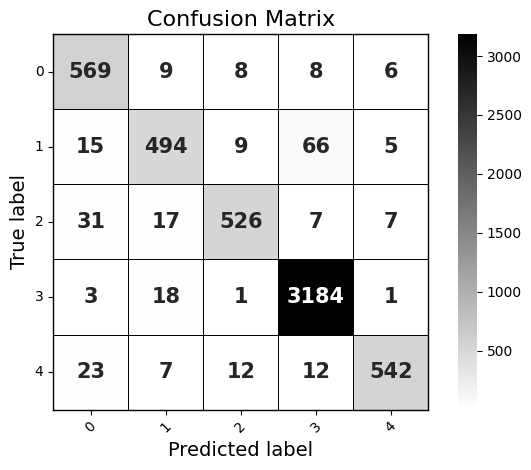
\includegraphics[width=0.8\textwidth]{Images/SVM Confusion Matrix.png}  
    \caption{Confusion Matrix (SVM)}
    \label{SVMCM}  % Label for referencing the figure
\end{figure}

\noindent
The Support Vector Machine (SVM) model achieved an accuracy of 85.13\%, demonstrating strong performance in classifying the various mental health conditions. The classification report indicates that the Normal class has the highest precision (0.94) and recall (0.95), resulting in an F1-score of 0.95, showing that the model is particularly good at identifying instances of normal behavior. However, the Bipolar class shows lower performance, with a precision of 0.62 and recall of 0.61, suggesting that the model struggles more with identifying bipolar disorder instances. The recall for the Anxiety class is relatively high (0.76), though precision is somewhat lower (0.72), indicating a balanced classification performance for this condition. The confusion matrix reveals that the model is generally accurate, with the Normal class being correctly classified most of the time (2084 true positives). However, some misclassifications occur for classes like Bipolar, Depression, and PTSD, with notable misclassifications of Bipolar as Depression and Normal. These misclassifications are likely affecting the overall recall for certain classes. The ROC AUC curve areas demonstrate that the model has excellent performance in distinguishing between most classes. The Normal class has the highest AUC of 0.98, followed by Anxiety, Depression, and PTSD with AUCs of 0.96. Bipolar, although still high at 0.90, lags behind the other classes, reflecting the model's challenge in distinguishing Bipolar from other conditions.

\begin{figure}[h!]  
    \centering
    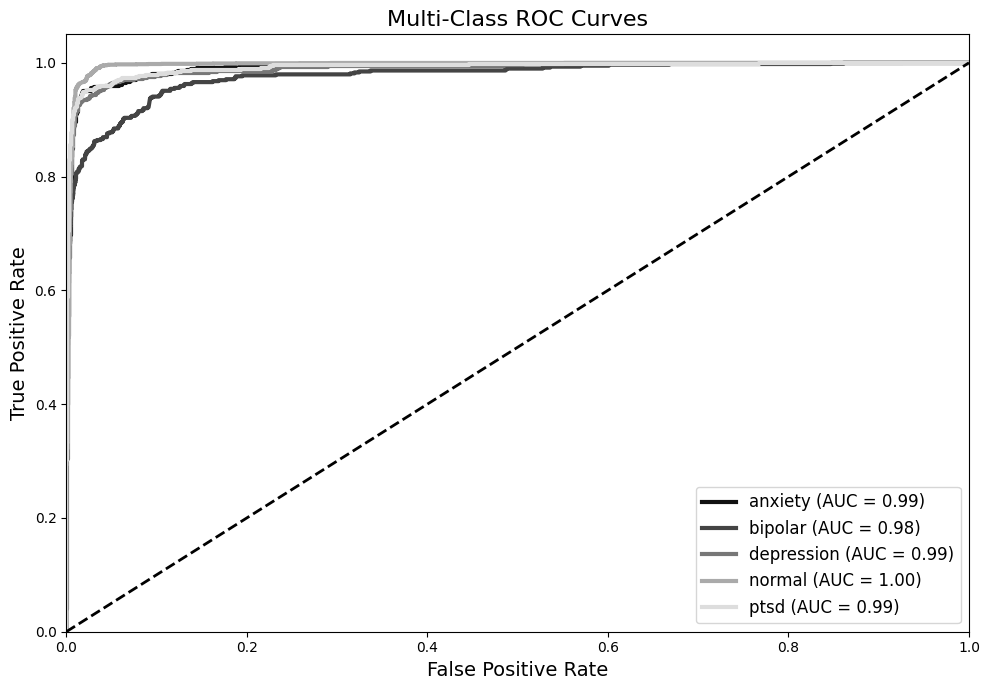
\includegraphics[width=0.75\textwidth]{Images/SVM ROC.png}  
    \caption{ROC AUC (SVM)}
    \label{SVMSOC}  % Label for referencing the figure
\end{figure}


\subsection{Results of Random Forest}

\begin{center}
    \textbf{Random Forest Classification Report} \\[0.5em]
    \begin{tabular}{|l|c|c|c|c|}
        \hline
        \textbf{Class} & \textbf{Precision} & \textbf{Recall} & \textbf{F1-Score} & \textbf{Support} \\ \hline
        Anxiety        & 0.81               & 0.70            & 0.75              & 379              \\ \hline
        Bipolar        & 0.93               & 0.47            & 0.62              & 384              \\ \hline
        Depression     & 0.72               & 0.77            & 0.74              & 373              \\ \hline
        Normal         & 0.88               & 1.00            & 0.93              & 2183             \\ \hline
        PTSD           & 0.92               & 0.74            & 0.82              & 394              \\ \hline
        \textbf{Accuracy} & \multicolumn{4}{|c|}{86.00\%} \\ \hline
        \textbf{Macro Avg} & 0.85            & 0.73            & 0.77              & 3713             \\ \hline
        \textbf{Weighted Avg} & 0.86         & 0.86            & 0.85              & 3713             \\ \hline
    \end{tabular}
\end{center}

\vspace{0.25em}

\begin{center}
    \textbf{Confusion Matrix for Random Forest Model} \\[0.5em]
    \begin{tabular}{|c|c|c|c|c|c|}
        \hline
        & \textbf{Anxiety} & \textbf{Bipolar} & \textbf{Depression} & \textbf{Normal} & \textbf{PTSD} \\ \hline
        \textbf{Anxiety}    & 264 & 3   & 34  & 68  & 10  \\ \hline
        \textbf{Bipolar}    & 12  & 180 & 46  & 141 & 5   \\ \hline
        \textbf{Depression} & 26  & 3   & 286 & 48  & 10  \\ \hline
        \textbf{Normal}     & 3   & 6   & 1   & 2173 & 0  \\ \hline
        \textbf{PTSD}       & 19  & 2   & 30  & 53  & 290 \\ \hline
    \end{tabular}
\end{center}

\vspace{0.25em}

\begin{center}
    \textbf{ROC Curve Areas for Each Class} \\[0.5em]
    \begin{tabular}{|l|c|}
        \hline
        \textbf{Class}  & \textbf{ROC AUC} \\ \hline
        Anxiety         & 0.96            \\ \hline
        Bipolar         & 0.89            \\ \hline
        Depression      & 0.97            \\ \hline
        Normal          & 0.97            \\ \hline
        PTSD            & 0.97            \\ \hline
    \end{tabular}
\end{center}

\vspace{0.25em}

\begin{figure}[h!]  
    \centering
    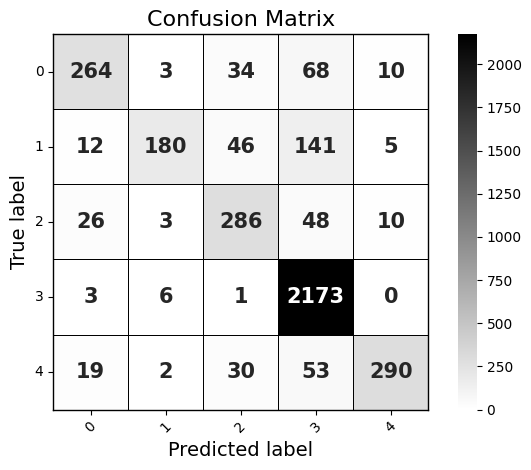
\includegraphics[width=0.8\textwidth]{Images/RF Confusion Matrix.png}  
    \caption{Confusion Matrix (Random Forest)}
    \label{RFCM}  % Label for referencing the figure
\end{figure}

\noindent
The Random Forest model achieved an accuracy of 86.00\%, indicating a strong performance in classifying the mental health conditions. The classification report shows that the Normal class achieved the highest recall (1.00) and a precision of 0.88, resulting in a high F1-score of 0.93. This reflects the model’s ability to correctly classify the majority of the Normal instances. The Bipolar class, however, shows a much lower recall (0.47), which indicates that the model has difficulty identifying instances of Bipolar disorder, as reflected by its F1-score of 0.62. The Anxiety and PTSD classes have relatively balanced performance, with moderate precision and recall values. The confusion matrix illustrates the distribution of misclassifications. The Normal class is correctly classified almost entirely (2173 true positives), while other classes like Bipolar and PTSD exhibit significant misclassifications, particularly Bipolar, which is often misclassified as Depression and Normal. The ROC AUC scores for all classes are quite high, indicating that the model is effective at distinguishing between the classes. The Anxiety, Depression, Normal, and PTSD classes each have AUC values above 0.96, with the Normal and Depression classes achieving 0.97. Bipolar has the lowest AUC at 0.89, which corresponds to its lower classification performance. These AUC values suggest that the Random Forest model is proficient in distinguishing between most of the classes, though it faces challenges in identifying Bipolar disorder.

\begin{figure}[h!]  
    \centering
    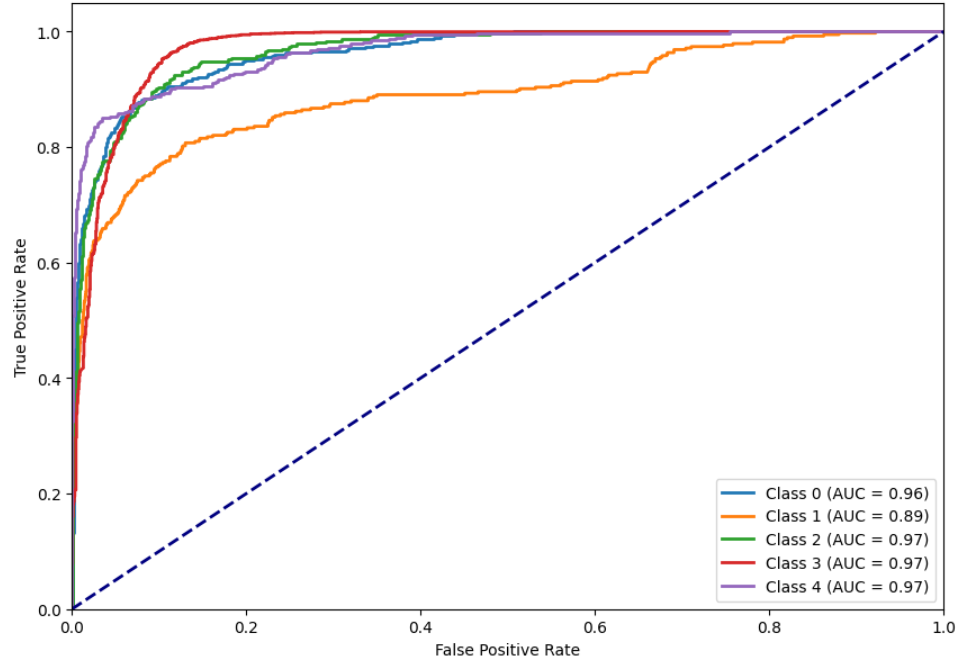
\includegraphics[width=0.7\textwidth]{Images/RF ROC.png}  
    \caption{ROC AUC (Random Forest)}
    \label{RFROC}  % Label for referencing the figure
\end{figure}


\subsection{Results of XGBoost}

\begin{center}
    \textbf{XGBoost Classification Report} \\[0.5em]
    \begin{tabular}{|l|c|c|c|c|}
        \hline
        \textbf{Class} & \textbf{Precision} & \textbf{Recall} & \textbf{F1-Score} & \textbf{Support} \\ \hline
        Anxiety        & 0.81               & 0.74            & 0.77              & 403              \\ \hline
        Bipolar        & 0.77               & 0.62            & 0.69              & 397              \\ \hline
        Depression     & 0.72               & 0.81            & 0.76              & 387              \\ \hline
        Normal         & 0.93               & 0.98            & 0.95              & 2137             \\ \hline
        PTSD           & 0.86               & 0.75            & 0.80              & 396              \\ \hline
        \textbf{Accuracy} & \multicolumn{4}{|c|}{87.39\%} \\ \hline
        \textbf{Macro Avg} & 0.82            & 0.78            & 0.80              & 3720             \\ \hline
        \textbf{Weighted Avg} & 0.87         & 0.87            & 0.87              & 3720             \\ \hline
    \end{tabular}
\end{center}

\vspace{0.25em}

\begin{center}
    \textbf{Confusion Matrix for XGBoost Model} \\[0.5em]
    \begin{tabular}{|c|c|c|c|c|c|}
        \hline
        & \textbf{Anxiety} & \textbf{Bipolar} & \textbf{Depression} & \textbf{Normal} & \textbf{PTSD} \\ \hline
        \textbf{Anxiety}    & 297 & 20  & 39  & 24  & 23  \\ \hline
        \textbf{Bipolar}    & 13  & 248 & 36  & 92  & 8   \\ \hline
        \textbf{Depression} & 30  & 13  & 313 & 17  & 14  \\ \hline
        \textbf{Normal}     & 3   & 28  & 8   & 2096 & 2   \\ \hline
        \textbf{PTSD}       & 22  & 12  & 36  & 29  & 297 \\ \hline
    \end{tabular}
\end{center}

\vspace{0.25em}

\begin{center}
    \textbf{ROC Curve Areas for Each Class} \\[0.5em]
    \begin{tabular}{|l|c|}
        \hline
        \textbf{Class}  & \textbf{ROC AUC} \\ \hline
        Anxiety         & 0.97            \\ \hline
        Bipolar         & 0.95            \\ \hline
        Depression      & 0.97            \\ \hline
        Normal          & 0.99            \\ \hline
        PTSD            & 0.97            \\ \hline
    \end{tabular}
\end{center}

\vspace{0.25em}

\noindent
The XGBoost model achieved an accuracy of 87.39\%, demonstrating strong overall performance. The classification report indicates high precision and recall for the 'Normal' class, which is likely due to its substantial representation in the dataset. The 'Anxiety' and 'PTSD' classes also showed reasonable results, with the 'Anxiety' class achieving a precision of 0.81 and a recall of 0.74. However, the 'Bipolar' class exhibited a lower recall (0.62), suggesting that the model struggles more with this class. The confusion matrix highlights a well-separated 'Normal' class, while the 'Bipolar' and 'PTSD' classes experience more confusion with other categories. The ROC AUC scores further emphasize the model's good discriminatory capability, with AUC values of 0.97 for 'Anxiety,' 'Depression,' and 'PTSD,' and 0.99 for 'Normal.' These scores indicate that the model is proficient at distinguishing between different mental health conditions in the dataset.

\begin{figure}[h!]  
    \centering
    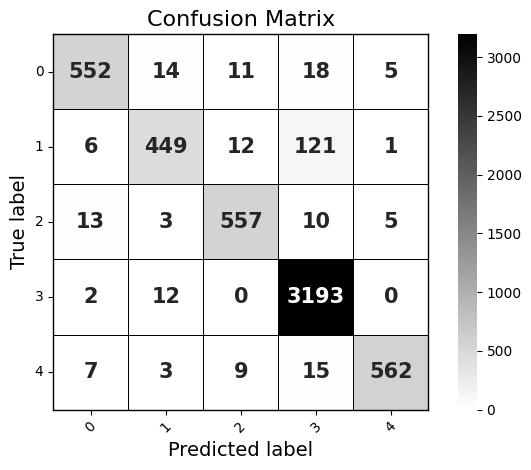
\includegraphics[width=0.85\textwidth]{Images/XG Confusion Matrix.png}  
    \caption{Confusion Matrix (XGBoost)}
    \label{XGCM}  % Label for referencing the figure
\end{figure}

\begin{figure}[h!]  
    \centering
    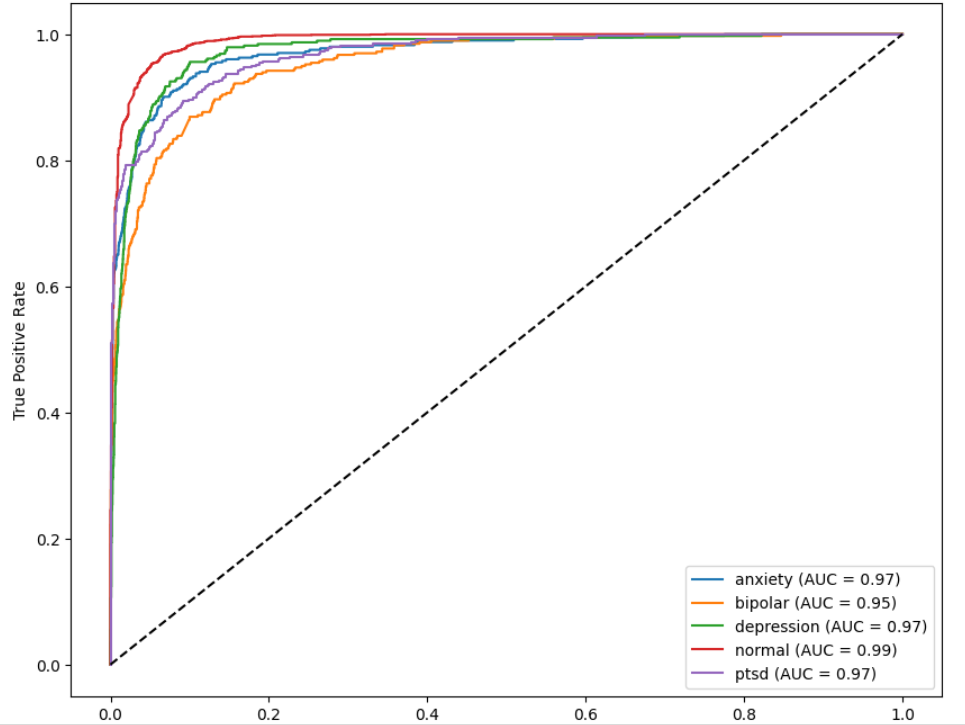
\includegraphics[width=0.85\textwidth]{Images/XG ROC.png}  
    \caption{ROC AUC (XGBoost)}
    \label{XGrOC}  % Label for referencing the figure
\end{figure}


\subsection{Results of KNN}

\begin{center}
    \textbf{KNN Classification Report} \\[0.5em]
    \begin{tabular}{|l|c|c|c|c|}
        \hline
        \textbf{Class} & \textbf{Precision} & \textbf{Recall} & \textbf{F1-Score} & \textbf{Support} \\ \hline
        Anxiety        & 0.58               & 0.31            & 0.40              & 379              \\ \hline
        Bipolar        & 0.18               & 0.59            & 0.28              & 384              \\ \hline
        Depression     & 0.47               & 0.39            & 0.43              & 373              \\ \hline
        Normal         & 0.79               & 0.69            & 0.73              & 2183             \\ \hline
        PTSD           & 0.80               & 0.09            & 0.16              & 394              \\ \hline
        \textbf{Accuracy} & \multicolumn{4}{|c|}{54.46\%} \\ \hline
        \textbf{Macro Avg} & 0.56            & 0.41            & 0.40              & 3713             \\ \hline
        \textbf{Weighted Avg} & 0.67         & 0.54            & 0.56              & 3713             \\ \hline
    \end{tabular}
\end{center}

\vspace{0.25em}

\begin{center}
    \textbf{Confusion Matrix for KNN Model} \\[0.5em]
    \begin{tabular}{|c|c|c|c|c|c|}
        \hline
        & \textbf{Anxiety} & \textbf{Bipolar} & \textbf{Depression} & \textbf{Normal} & \textbf{PTSD} \\ \hline
        \textbf{Anxiety}    & 117 & 122 & 35  & 101 & 4   \\ \hline
        \textbf{Bipolar}    & 7   & 226 & 40  & 108 & 3   \\ \hline
        \textbf{Depression} & 24  & 129 & 145 & 74  & 1   \\ \hline
        \textbf{Normal}     & 11  & 657 & 15  & 1499 & 1  \\ \hline
        \textbf{PTSD}       & 41  & 120 & 74  & 124 & 35  \\ \hline
    \end{tabular}
\end{center}

\vspace{0.25em}

\begin{center}
    \textbf{ROC Curve Areas for Each Class} \\[0.5em]
    \begin{tabular}{|l|c|}
        \hline
        \textbf{Class}  & \textbf{ROC AUC} \\ \hline
        Anxiety         & 0.73            \\ \hline
        Bipolar         & 0.67            \\ \hline
        Depression      & 0.77            \\ \hline
        Normal          & 0.80            \\ \hline
        PTSD            & 0.67            \\ \hline
    \end{tabular}
\end{center}

\vspace{0.25em}

\noindent
The KNN model achieved an accuracy of 54.46\%, which is considerably lower than the XGBoost model. The classification report reveals a significant imbalance in performance across classes. The 'Normal' class achieved relatively high precision (0.79) and recall (0.69), reflecting the model's tendency to perform well with dominant classes. However, the 'Anxiety' and 'PTSD' classes performed poorly, especially with PTSD having a very low recall of 0.09, indicating substantial misclassification. The confusion matrix suggests that the model struggles with distinguishing between some classes, especially 'Anxiety' and 'Bipolar,' where confusion with other categories is high. The ROC AUC scores are relatively lower compared to the XGBoost model, with 'Normal' having the highest AUC of 0.80. These results indicate that while the KNN model offers a lower overall performance, it still provides a reasonable level of discrimination for the 'Normal' class.

\begin{figure}[h!]  
    \centering
    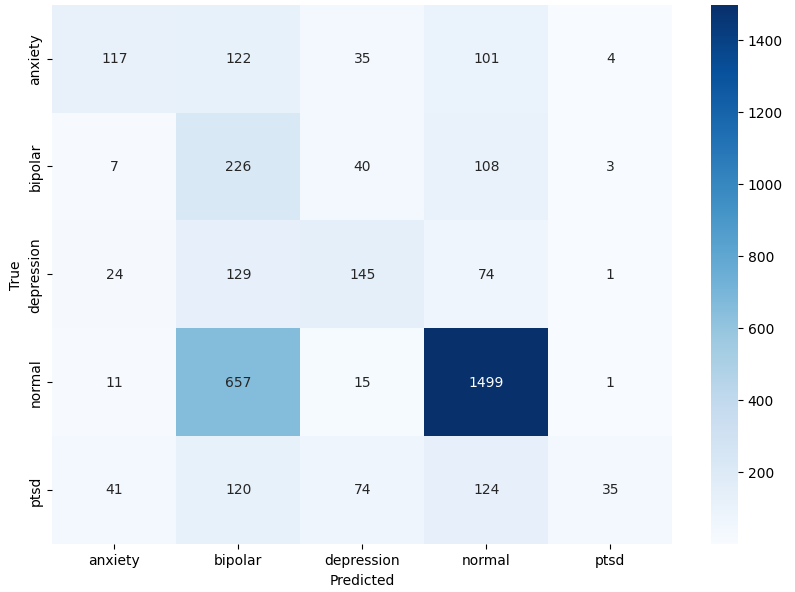
\includegraphics[width=0.85\textwidth]{Images/KNN Confusion Matrix.png}  
    \caption{Confusion Matrix (KNN)}
    \label{KNNCM}  % Label for referencing the figure
\end{figure}

\begin{figure}[h!]  
    \centering
    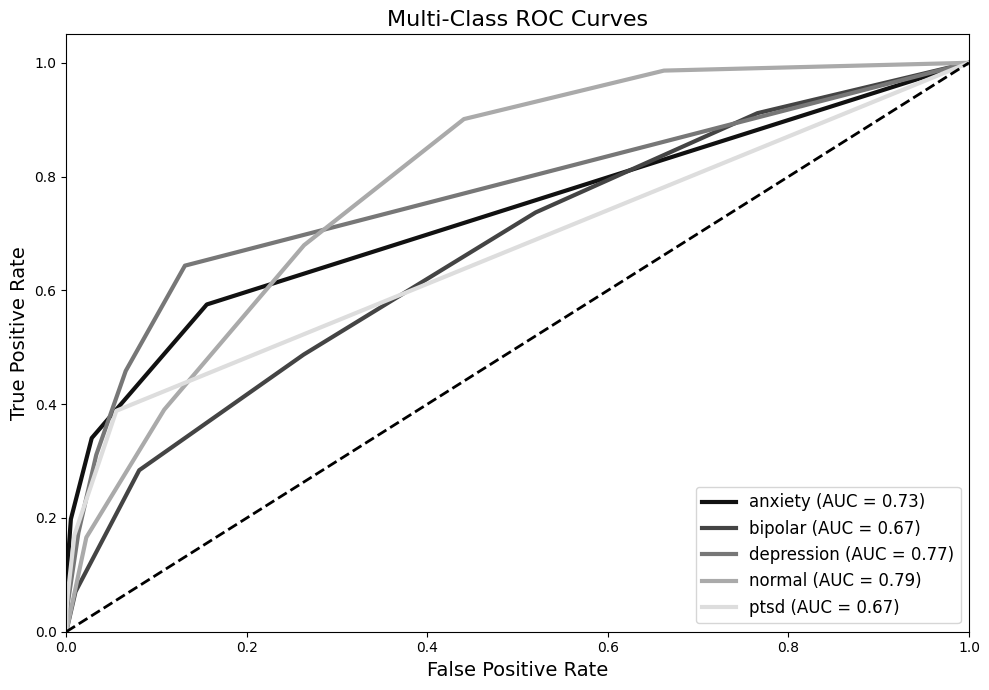
\includegraphics[width=0.8\textwidth]{Images/KNN ROC.png}  
    \caption{ROC AUC (KNN)}
    \label{KNnROC}  % Label for referencing the figure
\end{figure}



\subsection{Results of LSTM}

\begin{center}
    \textbf{LSTM Classification Report} \\[0.5em]
    \begin{tabular}{|l|c|c|c|c|}
        \hline
        \textbf{Class} & \textbf{Precision} & \textbf{Recall} & \textbf{F1-Score} & \textbf{Support} \\ \hline
        Anxiety        & 0.81               & 0.68            & 0.74              & 403              \\ \hline
        Bipolar        & 0.60               & 0.59            & 0.60              & 397              \\ \hline
        Depression     & 0.56               & 0.77            & 0.65              & 387              \\ \hline
        Normal         & 0.96               & 0.96            & 0.96              & 2137             \\ \hline
        PTSD           & 0.76               & 0.61            & 0.68              & 396              \\ \hline
        \textbf{Accuracy} & \multicolumn{4}{|c|}{83.55\%} \\ \hline
        \textbf{Macro Avg} & 0.74            & 0.72            & 0.73              & 3720             \\ \hline
        \textbf{Weighted Avg} & 0.84         & 0.84            & 0.84              & 3720             \\ \hline
    \end{tabular}
\end{center}

\vspace{0.25em}

\begin{center}
    \textbf{Confusion Matrix for LSTM Model} \\[0.5em]
    \begin{tabular}{|c|c|c|c|c|c|}
        \hline
        & \textbf{Anxiety} & \textbf{Bipolar} & \textbf{Depression} & \textbf{Normal} & \textbf{PTSD} \\ \hline
        \textbf{Anxiety}    & 274 & 36  & 32  & 28  & 33  \\ \hline
        \textbf{Bipolar}    & 26  & 233 & 42  & 85  & 11  \\ \hline
        \textbf{Depression} & 25  & 31  & 299 & 19  & 13  \\ \hline
        \textbf{Normal}     & 6   & 18  & 11  & 2043 & 9   \\ \hline
        \textbf{PTSD}       & 31  & 33  & 33  & 35  & 264 \\ \hline
    \end{tabular}
\end{center}

\vspace{0.25em}
\pagebreak

\begin{center}
    \textbf{ROC Curve Areas for Each Class} \\[0.5em]
    \begin{tabular}{|l|c|}
        \hline
        \textbf{Class}  & \textbf{ROC AUC} \\ \hline
        Anxiety         & 0.95            \\ \hline
        Bipolar         & 0.92            \\ \hline
        Depression      & 0.94            \\ \hline
        Normal          & 0.99            \\ \hline
        PTSD            & 0.95            \\ \hline
    \end{tabular}
\end{center}

\vspace{0.25em}

\noindent
The LSTM model achieved an accuracy of 83.55\%, indicating strong performance, although it lags slightly behind other models such as XGBoost and SVM. The classification report shows high precision, recall, and F1-scores for the 'Normal' class, which dominates the dataset. The 'Anxiety' class has reasonable performance, with a precision of 0.81 and recall of 0.68, but the 'Bipolar' and 'PTSD' classes have lower precision and recall, especially for 'Bipolar' (0.60 in both precision and recall). The confusion matrix reflects this, with 'Bipolar' and 'PTSD' misclassified with other classes, while 'Normal' is well-separated. The ROC AUC scores highlight the model's ability to distinguish between classes effectively, with 'Normal' scoring the highest AUC of 0.99, followed by other classes such as 'Anxiety' and 'Depression,' both with AUCs above 0.90.

\begin{figure}[h!]  
    \centering
    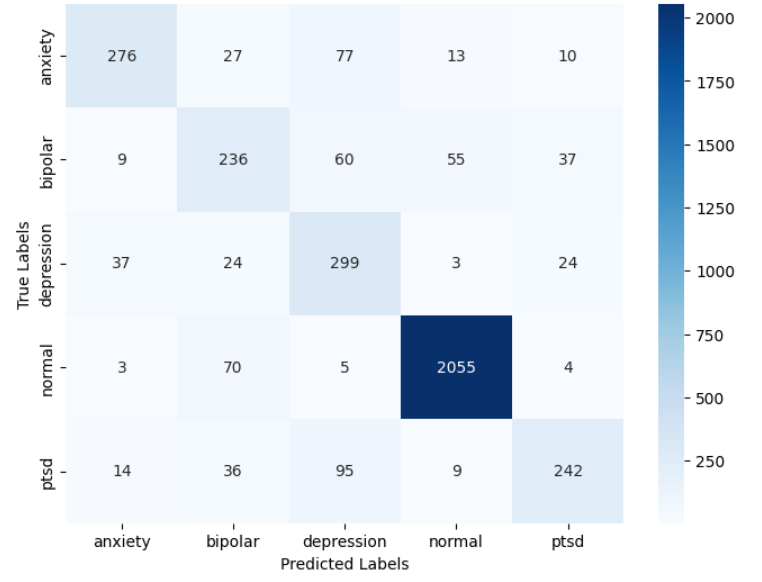
\includegraphics[width=0.85\textwidth]{Images/LSTM Confusion Matrix.png}  
    \caption{Confusion Matrix (LSTM)}
    \label{LSTMCM}  % Label for referencing the figure
\end{figure}

\begin{figure}[h!]  
    \centering
    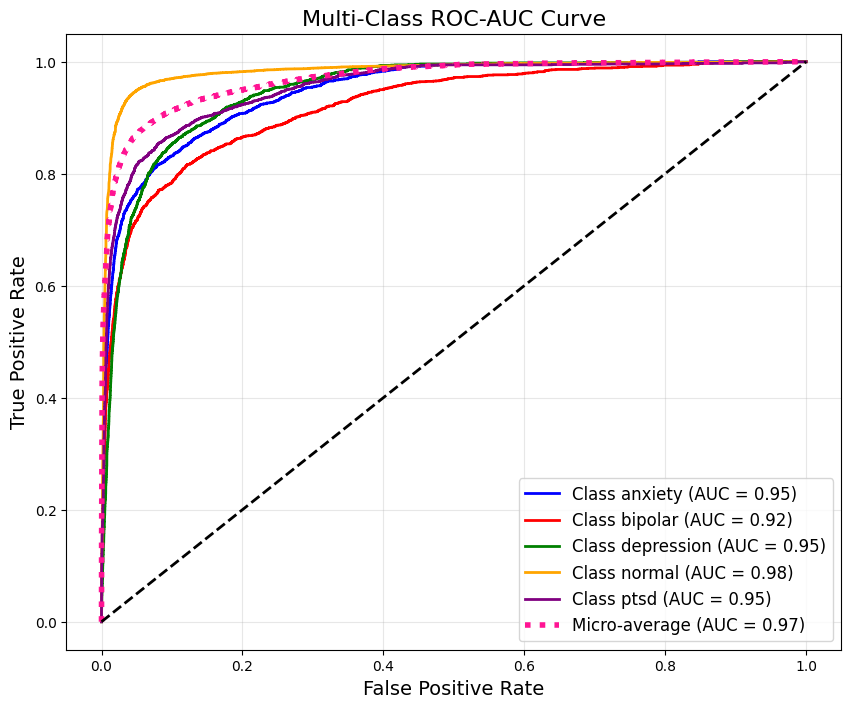
\includegraphics[width=0.8\textwidth]{Images/LSTM ROC.png}  
    \caption{ROC AUC (LSTM)}
    \label{LSTMROC}  % Label for referencing the figure
\end{figure}

\pagebreak
\noindent
Among the various machine learning algorithms tested, Logistic Regression emerged as the best performing model. With an accuracy of 87.66\%, it outperformed the other models in terms of overall accuracy, precision, recall, and F1-score. The classification report for Logistic Regression shows strong performance across all classes, especially the 'Normal' class, which had high precision (0.92) and recall (0.99). Although the model faced challenges with the 'Bipolar' class, which had lower recall and F1-score, its overall ability to differentiate between other mental health conditions was impressive. The confusion matrix and ROC AUC scores further highlight the model’s robustness, with an AUC of 0.99 for the 'Normal' class and strong values for other classes as well. This indicates that Logistic Regression not only achieves high accuracy but also performs well in distinguishing between different mental health categories, making it the most reliable choice for this classification task.

% ------------------------ Result and Analysis Ends -------------------------
